\documentclass{standalone}
\usepackage{tikz}
\usetikzlibrary{patterns, positioning}
\usepackage[sfdefault]{ClearSans} %% option 'sfdefault' activates Clear Sans as the default text font
\usepackage[T1]{fontenc}

\begin{document}
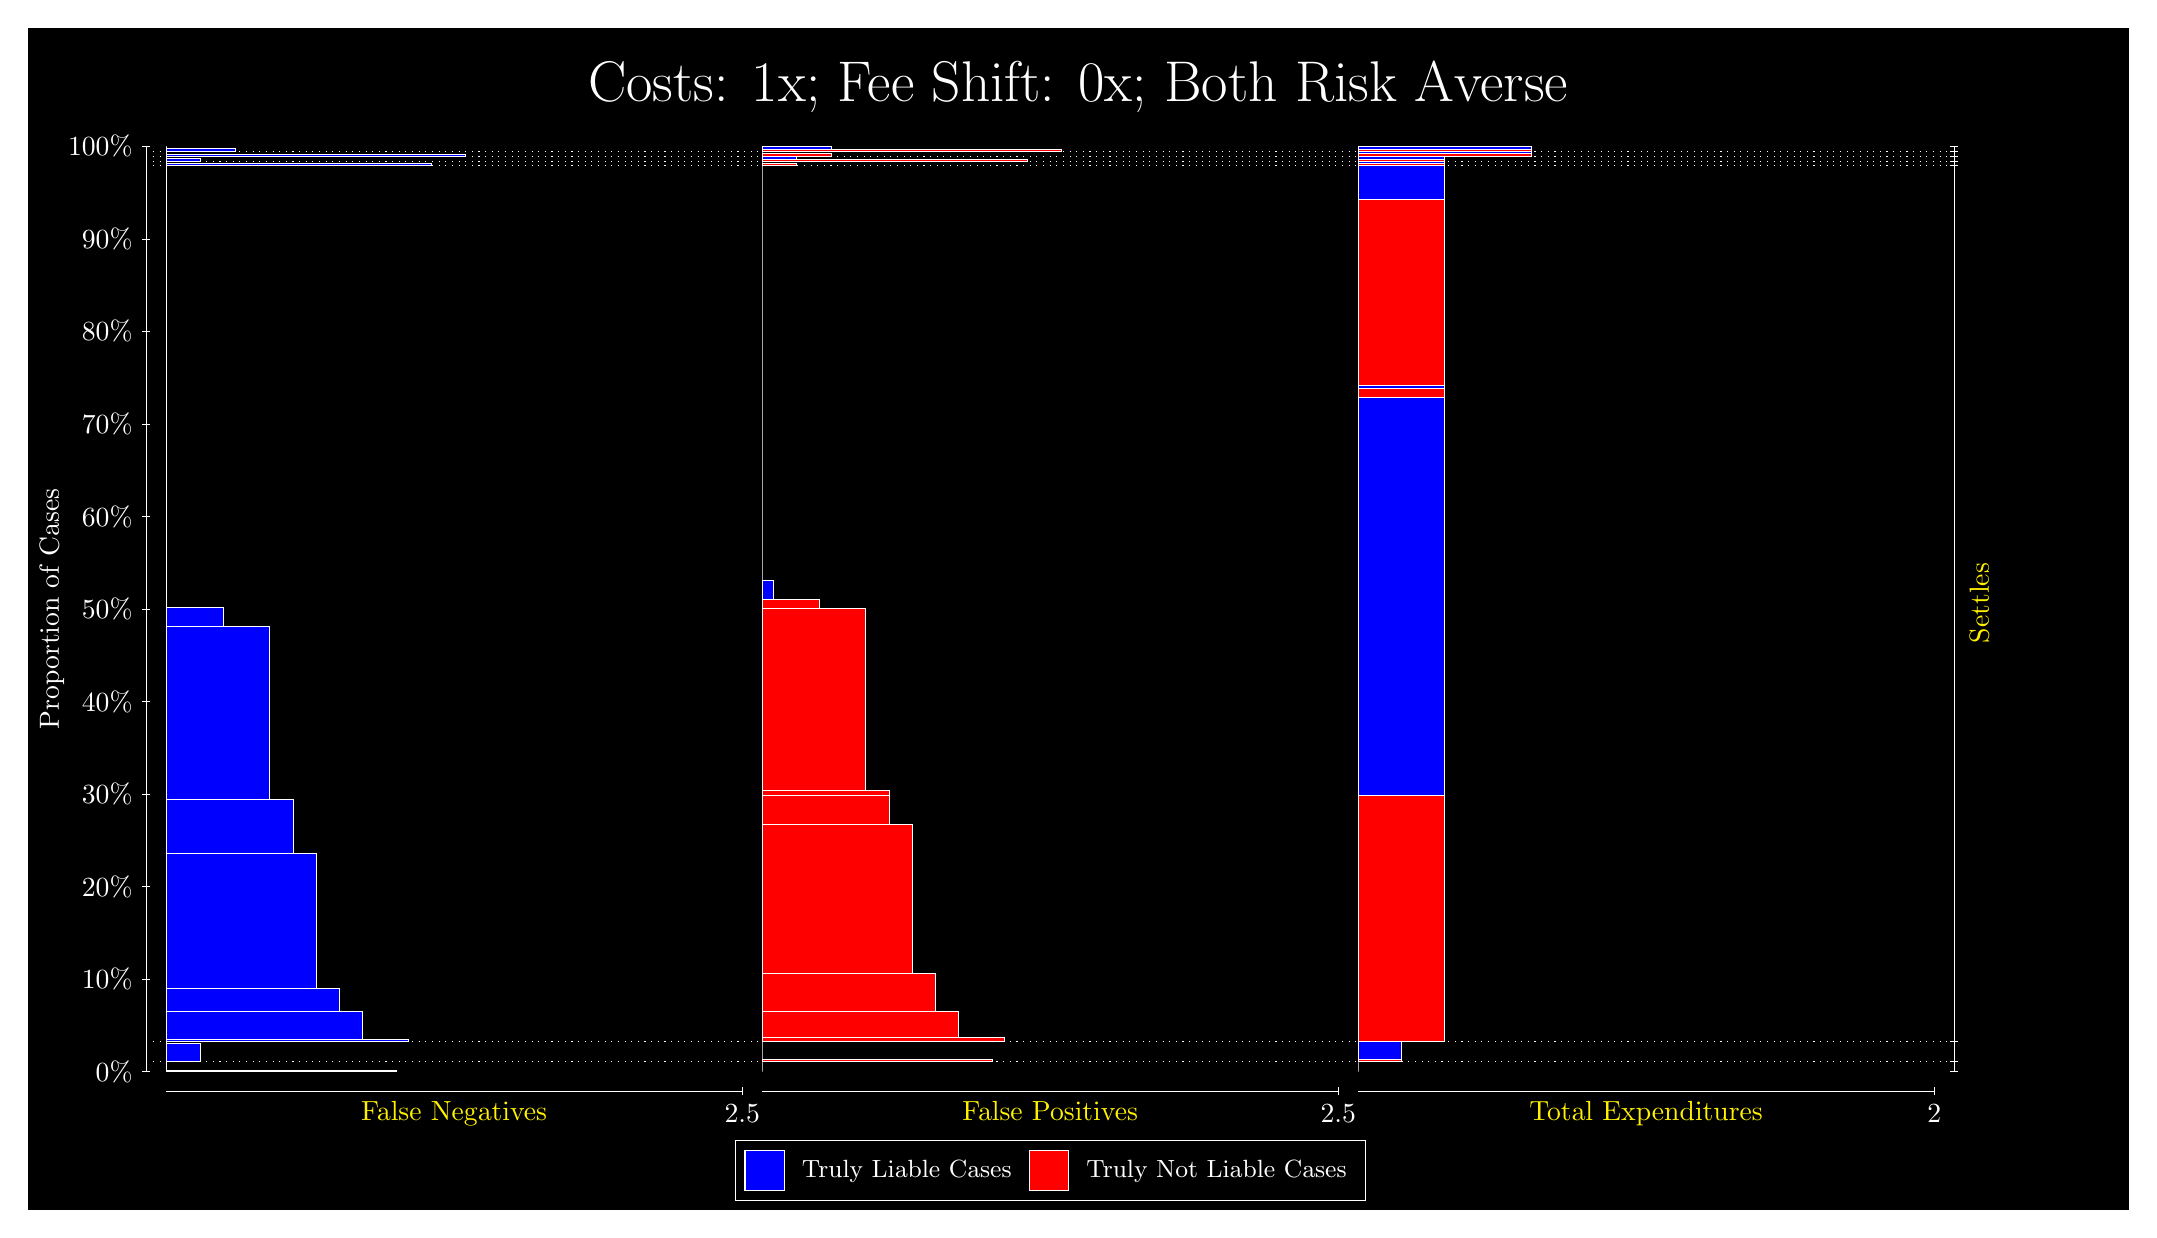
\begin{tikzpicture}
\draw[fill=black] (0,0) rectangle (26.667,15);
\draw[text=white] (0,13.5) rectangle (26.667,15) node[midway] {\huge Costs: 1x; Fee Shift: 0x; Both Risk Averse};
\draw[white, very thin] (1.5,1.75) -- (1.5,13.5);
\node[rotate=90, text=white, anchor=center] at (0.3, 7.625) {Proportion of Cases};
\draw[white, very thin] (1.45,1.75) -- (1.55,1.75);
\node[text=white, anchor=east] at (1.45, 1.75) {0\%};
\draw[white, very thin] (1.45,2.925) -- (1.55,2.925);
\node[text=white, anchor=east] at (1.45, 2.925) {10\%};
\draw[white, very thin] (1.45,4.1) -- (1.55,4.1);
\node[text=white, anchor=east] at (1.45, 4.1) {20\%};
\draw[white, very thin] (1.45,5.275) -- (1.55,5.275);
\node[text=white, anchor=east] at (1.45, 5.275) {30\%};
\draw[white, very thin] (1.45,6.45) -- (1.55,6.45);
\node[text=white, anchor=east] at (1.45, 6.45) {40\%};
\draw[white, very thin] (1.45,7.625) -- (1.55,7.625);
\node[text=white, anchor=east] at (1.45, 7.625) {50\%};
\draw[white, very thin] (1.45,8.8) -- (1.55,8.8);
\node[text=white, anchor=east] at (1.45, 8.8) {60\%};
\draw[white, very thin] (1.45,9.975) -- (1.55,9.975);
\node[text=white, anchor=east] at (1.45, 9.975) {70\%};
\draw[white, very thin] (1.45,11.15) -- (1.55,11.15);
\node[text=white, anchor=east] at (1.45, 11.15) {80\%};
\draw[white, very thin] (1.45,12.325) -- (1.55,12.325);
\node[text=white, anchor=east] at (1.45, 12.325) {90\%};
\draw[white, very thin] (1.45,13.5) -- (1.55,13.5);
\node[text=white, anchor=east] at (1.45, 13.5) {100\%};

\draw[white, very thin] (24.457,1.75) -- (24.457,13.5);
\draw[white, very thin] (24.407,1.75) -- (24.507,1.75);
\node[anchor=west] at (24.407, 1.75) {};
\draw[white, very thin] (24.407,1.8786) -- (24.507,1.8786);
\node[anchor=west] at (24.407, 1.8786) {};
\draw[white, very thin] (24.407,2.1358) -- (24.507,2.1358);
\node[anchor=west] at (24.407, 2.1358) {};
\draw[white, very thin] (24.407,13.262) -- (24.507,13.262);
\node[anchor=west] at (24.407, 13.262) {};
\draw[white, very thin] (24.407,13.305) -- (24.507,13.305);
\node[anchor=west] at (24.407, 13.305) {};
\draw[white, very thin] (24.407,13.373) -- (24.507,13.373);
\node[anchor=west] at (24.407, 13.373) {};
\draw[white, very thin] (24.407,13.437) -- (24.507,13.437);
\node[anchor=west] at (24.407, 13.437) {};
\draw[white, very thin] (24.407,13.5) -- (24.507,13.5);
\node[anchor=west] at (24.407, 13.5) {};

\draw[white, very thin, fill=blue] (1.75,1.75) rectangle (4.6775,1.7635);
\draw[white, very thin, fill=red] (1.75,1.7635) rectangle (1.75,1.8786);
\draw[white, very thin, fill=blue] (1.75,1.8786) rectangle (2.1891,2.1087);
\draw[white, very thin, fill=red] (1.75,2.1087) rectangle (1.75,2.1358);
\draw[white, very thin, fill=blue] (1.75,2.1358) rectangle (4.8239,2.1621);
\draw[white, very thin, fill=blue] (1.75,2.1621) rectangle (4.2384,2.5159);
\draw[white, very thin, fill=blue] (1.75,2.5159) rectangle (3.9457,2.8058);
\draw[white, very thin, fill=blue] (1.75,2.8058) rectangle (3.6529,4.516);
\draw[white, very thin, fill=blue] (1.75,4.516) rectangle (3.3602,5.2035);
\draw[white, very thin, fill=blue] (1.75,5.2035) rectangle (3.0674,7.4071);
\draw[white, very thin, fill=blue] (1.75,7.4071) rectangle (2.4819,7.6469);
\draw[white, very thin, fill=red] (1.75,7.6469) rectangle (1.75,13.262);
\draw[white, very thin, fill=blue] (1.75,13.262) rectangle (5.1167,13.279);
\draw[white, very thin, fill=red] (1.75,13.279) rectangle (1.75,13.305);
\draw[white, very thin, fill=blue] (1.75,13.305) rectangle (2.1891,13.344);
\draw[white, very thin, fill=red] (1.75,13.344) rectangle (1.75,13.373);
\draw[white, very thin, fill=blue] (1.75,13.373) rectangle (5.5558,13.395);
\draw[white, very thin, fill=red] (1.75,13.395) rectangle (1.75,13.437);
\draw[white, very thin, fill=blue] (1.75,13.437) rectangle (2.6283,13.478);
\draw[white, very thin, fill=red] (1.75,13.478) rectangle (1.75,13.5);
\draw[white, very thin, fill=red] (9.3189,1.75) rectangle (9.3189,1.8651);
\draw[white, very thin, fill=blue] (9.3189,1.8651) rectangle (9.3189,1.8786);
\draw[white, very thin, fill=red] (9.3189,1.8786) rectangle (12.246,1.9057);
\draw[white, very thin, fill=blue] (9.3189,1.9057) rectangle (9.3189,2.1358);
\draw[white, very thin, fill=red] (9.3189,2.1358) rectangle (12.393,2.1884);
\draw[white, very thin, fill=red] (9.3189,2.1884) rectangle (11.807,2.5192);
\draw[white, very thin, fill=red] (9.3189,2.5192) rectangle (11.515,2.993);
\draw[white, very thin, fill=red] (9.3189,2.993) rectangle (11.222,4.8858);
\draw[white, very thin, fill=red] (9.3189,4.8858) rectangle (10.929,5.2599);
\draw[white, very thin, fill=red] (9.3189,5.2599) rectangle (10.929,5.3231);
\draw[white, very thin, fill=red] (9.3189,5.3231) rectangle (10.636,7.6306);
\draw[white, very thin, fill=red] (9.3189,7.6306) rectangle (10.051,7.7505);
\draw[white, very thin, fill=blue] (9.3189,7.7505) rectangle (9.4652,7.9904);
\draw[white, very thin, fill=blue] (9.3189,7.9904) rectangle (9.3189,13.262);
\draw[white, very thin, fill=red] (9.3189,13.262) rectangle (9.758,13.287);
\draw[white, very thin, fill=blue] (9.3189,13.287) rectangle (9.3189,13.305);
\draw[white, very thin, fill=red] (9.3189,13.305) rectangle (12.686,13.333);
\draw[white, very thin, fill=blue] (9.3189,13.333) rectangle (9.758,13.373);
\draw[white, very thin, fill=red] (9.3189,13.373) rectangle (10.197,13.415);
\draw[white, very thin, fill=blue] (9.3189,13.415) rectangle (9.3189,13.437);
\draw[white, very thin, fill=red] (9.3189,13.437) rectangle (13.125,13.459);
\draw[white, very thin, fill=blue] (9.3189,13.459) rectangle (10.197,13.5);
\draw[white, very thin, fill=red] (16.888,1.75) rectangle (16.888,1.8651);
\draw[white, very thin, fill=blue] (16.888,1.8651) rectangle (16.888,1.8786);
\draw[white, very thin, fill=red] (16.888,1.8786) rectangle (17.437,1.9057);
\draw[white, very thin, fill=blue] (16.888,1.9057) rectangle (17.437,2.1358);
\draw[white, very thin, fill=red] (16.888,2.1358) rectangle (17.986,5.2599);
\draw[white, very thin, fill=blue] (16.888,5.2599) rectangle (17.986,10.313);
\draw[white, very thin, fill=red] (16.888,10.313) rectangle (17.986,10.433);
\draw[white, very thin, fill=blue] (16.888,10.433) rectangle (17.986,10.459);
\draw[white, very thin, fill=red] (16.888,10.459) rectangle (17.986,12.83);
\draw[white, very thin, fill=blue] (16.888,12.83) rectangle (17.986,13.262);
\draw[white, very thin, fill=red] (16.888,13.262) rectangle (17.986,13.287);
\draw[white, very thin, fill=blue] (16.888,13.287) rectangle (17.986,13.305);
\draw[white, very thin, fill=red] (16.888,13.305) rectangle (17.986,13.333);
\draw[white, very thin, fill=blue] (16.888,13.333) rectangle (17.986,13.373);
\draw[white, very thin, fill=red] (16.888,13.373) rectangle (19.083,13.415);
\draw[white, very thin, fill=blue] (16.888,13.415) rectangle (19.083,13.437);
\draw[white, very thin, fill=red] (16.888,13.437) rectangle (19.083,13.459);
\draw[white, very thin, fill=blue] (16.888,13.459) rectangle (19.083,13.5);
\draw[white, dotted] (1.5,1.8786) -- (24.457,1.8786);
\draw[white, dotted] (1.5,2.1358) -- (24.457,2.1358);
\draw[white, dotted] (1.5,13.262) -- (24.457,13.262);
\draw[white, dotted] (1.5,13.305) -- (24.457,13.305);
\draw[white, dotted] (1.5,13.373) -- (24.457,13.373);
\draw[white, dotted] (1.5,13.437) -- (24.457,13.437);
\draw[white, very thin] (1.75,1.5) -- (9.0689,1.5);
\node[text=yellow, anchor=north] at (5.4094, 1.5) {False Negatives};
\draw[white, very thin] (9.0689,1.45) -- (9.0689,1.55);
\node[text=white, anchor=north] at (9.0689, 1.45) {2.5};

\draw[white, very thin] (9.3189,1.5) -- (16.638,1.5);
\node[text=yellow, anchor=north] at (12.978, 1.5) {False Positives};
\draw[white, very thin] (16.638,1.45) -- (16.638,1.55);
\node[text=white, anchor=north] at (16.638, 1.45) {2.5};

\draw[white, very thin] (16.888,1.5) -- (24.207,1.5);
\node[text=yellow, anchor=north] at (20.547, 1.5) {Total Expenditures};
\draw[white, very thin] (24.207,1.45) -- (24.207,1.55);
\node[text=white, anchor=north] at (24.207, 1.45) {2};



\node[text=yellow, centered, rotate=90] at (24.777, 7.6987) {Settles};





\draw (12.978300999999998,1.5) node[draw=none] (baseCoordinate) {};
\begin{scope}[align=center]
        \matrix[scale=0.5, draw=white, below=0.5cm of baseCoordinate, nodes={draw}, column sep=0.1cm]{
            \node[rectangle, draw, minimum width=0.5cm, minimum height=0.5cm, fill=blue] {}; &
            \node[draw=none, font=\small, text=white] (B) {Truly Liable Cases}; &
            \node[rectangle, draw, minimum width=0.5cm, minimum height=0.5cm, fill=red] {}; &
            \node[draw=none, font=\small, text=white] (B) {Truly Not Liable Cases}; \\
            };
\end{scope}

\end{tikzpicture}
\end{document}